\documentclass{article}
\usepackage[utf8]{inputenc}
\usepackage{amsmath}
\usepackage{graphicx}
\usepackage{geometry}
\usepackage{float}
\geometry{a4paper, margin=1in}

\title{Homework 6 - Part 1b: 1D Wedge Bearing Verification}
\author{}
\date{}

\begin{document}
\maketitle

\section*{Problem Setup}
To verify the finite element solver against the analytical solution for a 1D wedge bearing, the physical parameters were adjusted to represent a pure wedge. Specifically, the leading taper angle was set to zero ($T_a = 0$), and Neumann boundary conditions were enforced on the top and bottom edges of the domain. This was achieved by applying Dirichlet boundary conditions ($p=0$) exclusively to the leading ($x=0$) and trailing ($x=L$) edges, thus forcing a strictly 1D flow in the $x$-direction.

The analytical solution for the 1D wedge bearing is given by:
\begin{equation}
    \tilde{p}(x) = \frac{\alpha\Lambda}{1-\alpha^2}\left(\frac{1}{H^2} - \frac{1}{\alpha^2}\right) - \frac{\Lambda}{1-\alpha}\left(\frac{1}{H} - \frac{1}{\alpha}\right)
\end{equation}
where $\alpha = h_1/h_2$, $H(x) = \alpha + (1-\alpha)(x/L)$, and $\Lambda = 6\mu UL/h_2^2$.

\section*{Convergence Study Results}
A mesh refinement study was performed by varying the number of elements in the $x$-direction ($E_x \in \{15, 30, 60, 120\}$) while keeping $E_y = 40$ constant. The maximum pointwise error between the numerical solution $p(x)$ and the analytical solution $\tilde{p}(x)$ was computed for each mesh resolution.

\begin{table}[H]
    \centering
    \begin{tabular}{|c|c|}
        \hline
        \textbf{Number of Elements ($E_x$)} & \textbf{Max Pointwise Error} \\
        \hline
        15  & 2932.079 \\
        30  & 757.7912 \\
        60  & 201.5704 \\
        120 & 56.73146 \\
        \hline
    \end{tabular}
    \caption{Maximum pointwise error in $p(x)$ for different mesh resolutions.}
    \label{tab:convergence_data}
\end{table}

The estimated convergence rate, calculated from the slope of the log-log plot of the error versus $E_x$, is approximately \textbf{$-1.90$}. This value is close to $-2.0$, successfully demonstrating the expected second-order convergence of the linear triangular elements for this problem.

\section*{Figures}
Figure \ref{fig:pressure_1d} shows the pressure distribution, while Figure \ref{fig:convergence} illustrates the convergence behavior of the finite element solver.

\begin{figure}[H]
    \centering
    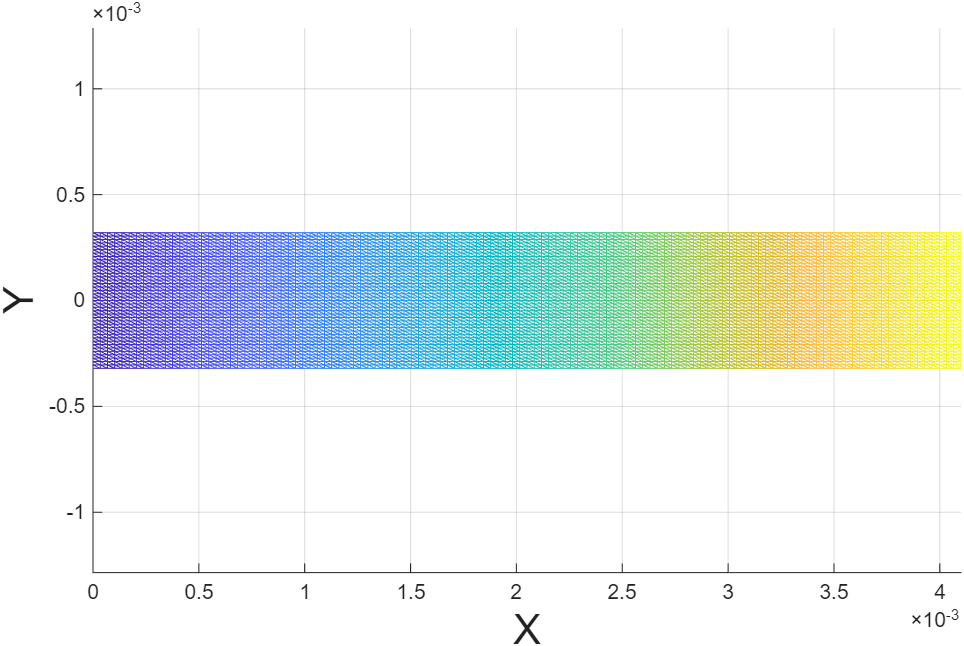
\includegraphics[width=0.8\textwidth]{part_1b_1}
    \caption{Numerical pressure profile for the 1D wedge bearing setup.}
    \label{fig:pressure_1d}
\end{figure}

\begin{figure}[H]
    \centering
    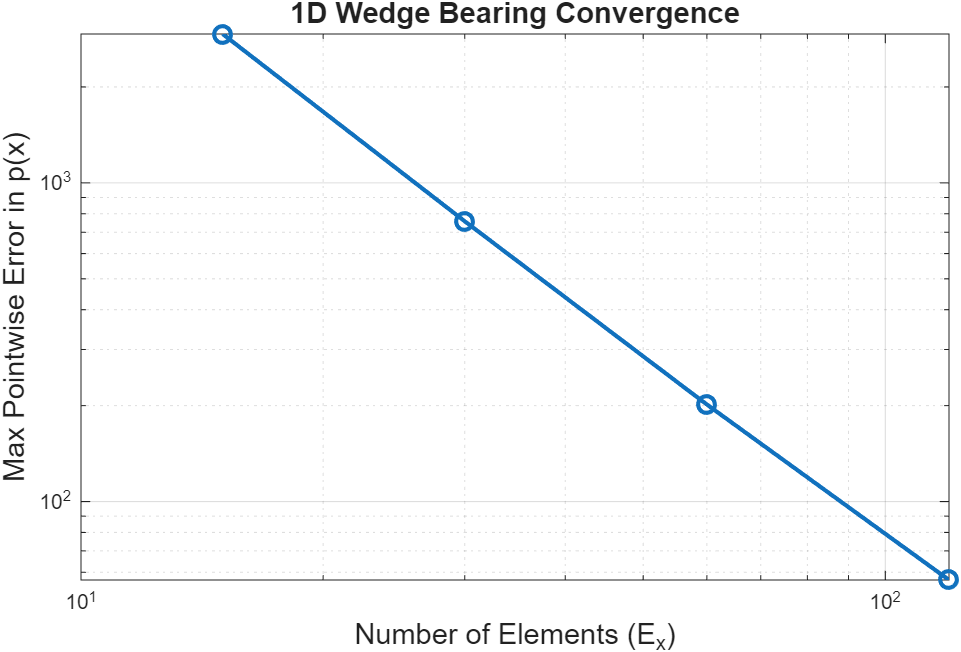
\includegraphics[width=0.8\textwidth]{part_1b_2}
    \caption{Log-log plot of the maximum pointwise error versus the number of elements ($E_x$), demonstrating near second-order convergence with a slope of $-1.90$.}
    \label{fig:convergence}
\end{figure}

\end{document}